\documentclass{beamer}
 
\usetheme{Madrid}
\makeatletter
\newcommand{\rmnum}[1]{\romannumeral #1}
\newcommand{\Rmnum}[1]{\expandafter\@slowromancap\romannumeral #1@}
\makeatother
 
%Information to be included in the title page:
\title[About Beamer] %optional
{Fused Deep Learning For Hurricane Track Forecast From Reanalysis Data}


\author{Mo YANG}


\institute[u-psud] % Your institution as it will appear on the bottom of every slide, may be shorthand to save space
{
	Supervisor: \\ % Your institution for the title page
	\medskip
	Claire Monteleoni
	\\
	Guillaume Charpiat 
	\\
	Sophie Giffard-Roison
}
\date{\today} % Date, can be changed to a custom date
 
 
 
\begin{document}

\begin{frame}
\titlepage % Print the title page as the first slide
\end{frame}


%----------------------------------------------------------------------------------------
%	PRESENTATION SLIDES
%----------------------------------------------------------------------------------------

%------------------------------------------------
\section{Background} % Sections can be created in order to organize your presentation into discrete blocks, all sections and subsections are automatically printed in the table of contents as an overview of the talk
%------------------------------------------------
\subsection{Hurricane Track Forecast}

\begin{frame}
\frametitle{Outline} % Table of contents slide, comment this block out to remove it
\tableofcontents[currentsection] % Throughout your presentation, if you choose to use \section{} and \subsection{} commands, these will automatically be printed on this slide as an overview of your presentation
\end{frame}


\begin{frame}
\frametitle{Hurricane}
\begin{itemize}
\item Cyclones, hurricanes or typhoons: words for the same phenomena
\item Cost tremendous damage and death each year
\item Can be very unpredictable.
\item \textbf{Tracks} and \textbf{Intensity} : Two main goals of the forecast
\end{itemize}
\end{frame}

\begin{frame}
\frametitle{Hurricane}
\begin{itemize}
	\item How hurricane is formed \\
\end{itemize}
\begin{figure}
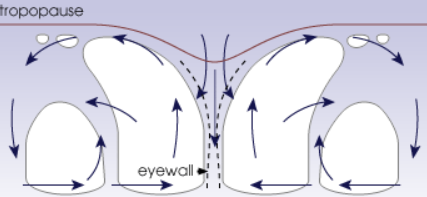
\includegraphics[width=0.8\linewidth]{figs/hurricane_section.png}
\end{figure}
\end{frame}

\begin{frame}
\frametitle{Hurricane}
\begin{itemize}
	\item The evolution and path of the hurricane Katrina (2005) \\
\end{itemize}
\begin{figure}
	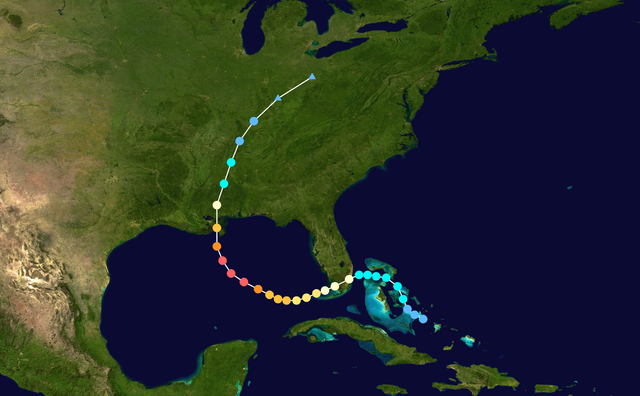
\includegraphics[width=0.6\linewidth, height=0.6\textheight]{figs/Katrina.png}
	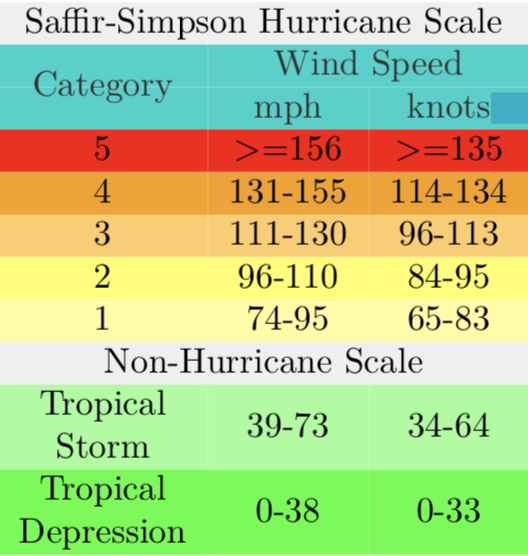
\includegraphics[width=0.3\linewidth, height=0.4\textheight]{figs/saffir-simpson.png}
\end{figure}
\end{frame}



\subsection{Hurricane Track Forecasting Models for Meteorologists }



\begin{frame}
\frametitle{Guidance Models}
\begin{itemize}
	\item Statistical models: do not consider physics, generate forecast in seconds. e.g. Best Track Decay (BCD5)
	\item Dynamic models: solve the physical equations governing the motions in the atmosphere, more accurate but computationally demanding. 
	\item Official NHC forecast (OFCL) :  consensus models which are created by combining the forecasts from a collection of other models.
\end{itemize}
\end{frame}
 

 
\section{Preliminaries}
\begin{frame}
\frametitle{Outline} % Table of contents slide, comment this block out to remove it
\tableofcontents[currentsection] % Throughout your presentation, if you choose to use \section{} and \subsection{} commands, these will automatically be printed on this slide as an overview of your presentation
\end{frame}

\subsection{Problem Setting}
\begin{frame}
\frametitle{Problem Setting}
\begin{itemize}
	\item Goal: estimating the 24h-forecast trajectory of all tropical storms.  \\
\end{itemize}
\begin{figure}
	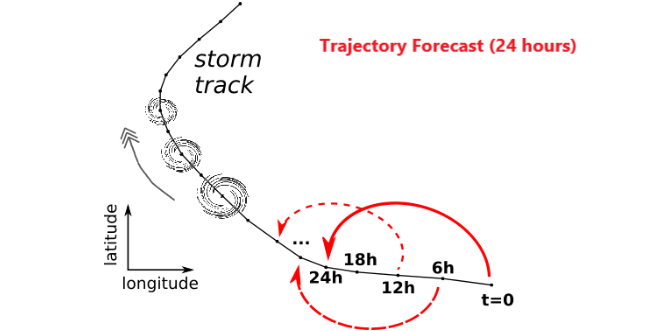
\includegraphics[width=0.8\linewidth]{figs/storm_shema.png}
\end{figure}
\end{frame}

\subsection{Previous Works}

\begin{frame}
\frametitle{Previous Works}
\begin{itemize}
\item A large family of previous methods use spatio-temporal features
\begin{itemize}
	\item Convolutional LSTM \cite{xingjian2015convolutional}
	\item Temporal Convolutional Networks \cite{bai2018empirical}
\end{itemize}
\item Only two preliminary studies have tackled the hurricane forecast tracking using machine learning
\begin{itemize}
	\item Use random forests on local reanalysis histograms \cite{liberge2011prevision}
	\item Train a sparse recurrent neural network from trajectory data \cite{moradi2016sparse}
\end{itemize}

\end{itemize}
\end{frame}
 
 \section{Method}
 \begin{frame}
 \frametitle{Outline} % Table of contents slide, comment this block out to remove it
 \tableofcontents[currentsection] % Throughout your presentation, if you choose to use \section{} and \subsection{} commands, these will automatically be printed on this slide as an overview of your presentation
\end{frame}
\subsection{Data Description}
\begin{frame}
\frametitle{Data}
\begin{itemize}
	\item  \textbf{Storm track data}: composed of tropical/extra-tropical storm tracks since 1979 extracted from the NOAA database IBTrACS. \\
\end{itemize}
\begin{figure}
	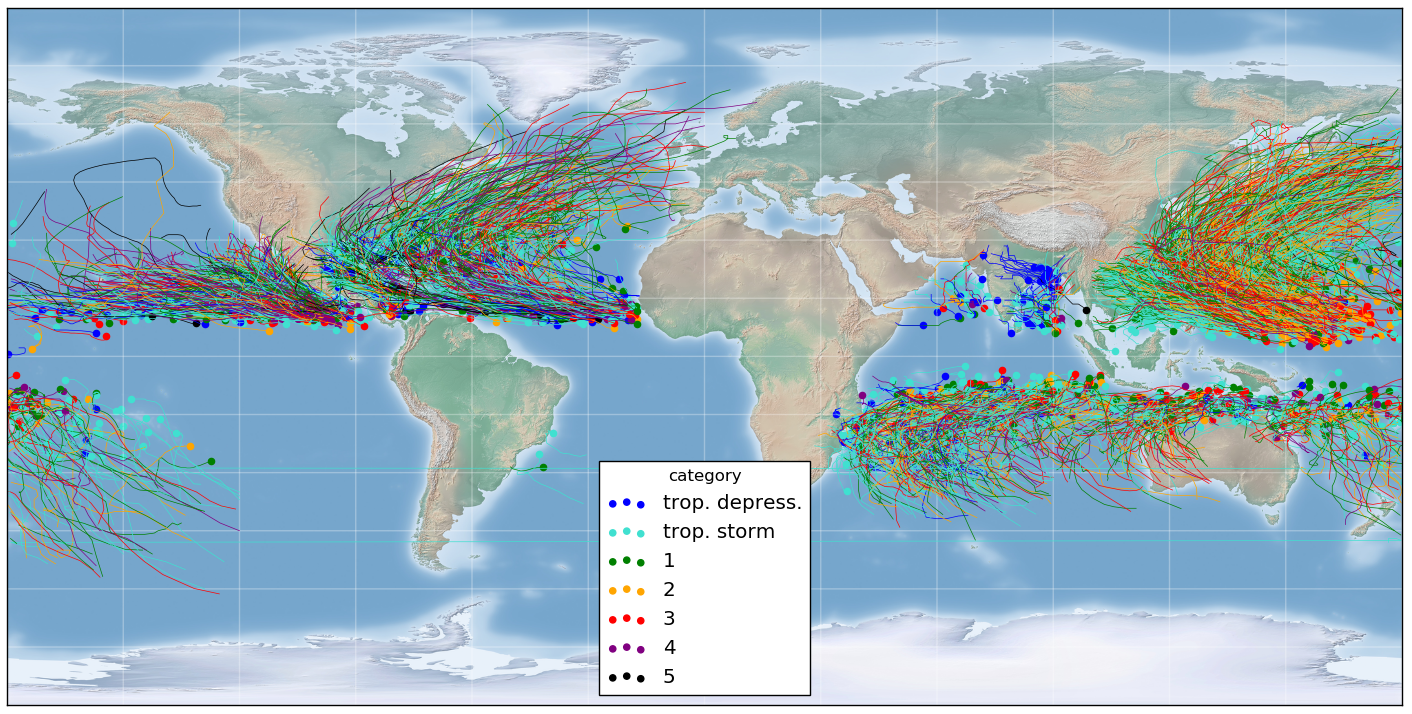
\includegraphics[width=0.7\linewidth, height=0.5\textheight]{figs/all_storms.png}
	\label{fig: storm_tracks}
	\caption{Database: tropical/extra-tropical storm tracks since 1979. Dots = initial position, colors = maximal storm strength according to the Saffir-Simpson scale.}
\end{figure}
\end{frame}

\begin{frame}
\frametitle{Data}
\begin{itemize}
	\item  \textbf{Reanalysis}: dynamically consistent estimates of the climate atmospheric fields or state. Created via data assimilation scheme and model(s) which take all available observations (radiosonde, satellite, buoy, aircraft and ship reports ...) as inputs every 6 hours.
	\item ERA-Interim: the latest global atmospheric reanalysis produced by The European Centre for Medium-Range Weather Forecasts (ECMWF). 
	\begin{itemize}
		\item spectral resolution: about 80km on 60 vertical levels from the surface up to 0.1 hPa
		\item atmospheric fields: u-wind, v-wind, pressure, temporature, humiity, vorticity ......
	\end{itemize}
\end{itemize}
\end{frame}

\subsection{Feature Selection}
\begin{frame}
\frametitle{Feature Selection}
\begin{itemize}
	\item \textbf{The wind fields.} u-wind and v-wind fields on a 25x25 degree grid centered on the current storm location, at three atmospheric pressure levels (700 hPa, 500 hPa, and 225 hPa). 
	\item \textbf{The pressure fields.} geopotential height fields on a 25x25 degree grid centered on the current storm location, at three atmospheric pressure levels (700 hPa, 500 hPa, and 225 hPa)
	\item \textbf{Displacement in history.} 
	\item \textbf{Other hand-crafted features:} current lat. \& lon.,  windspeed, Jday predictor(Gaussian function of "Julian day of storm init - peak day of the hurricane season"\cite{demaria2005further}), and current distance to land. 
	
\end{itemize}
\end{frame}

\subsection{The proposed method}
\begin{frame}
\frametitle{Overview of the proposed method}
\begin{itemize}
	\item  Three-stream fusion network \\
\end{itemize}
\begin{figure}
	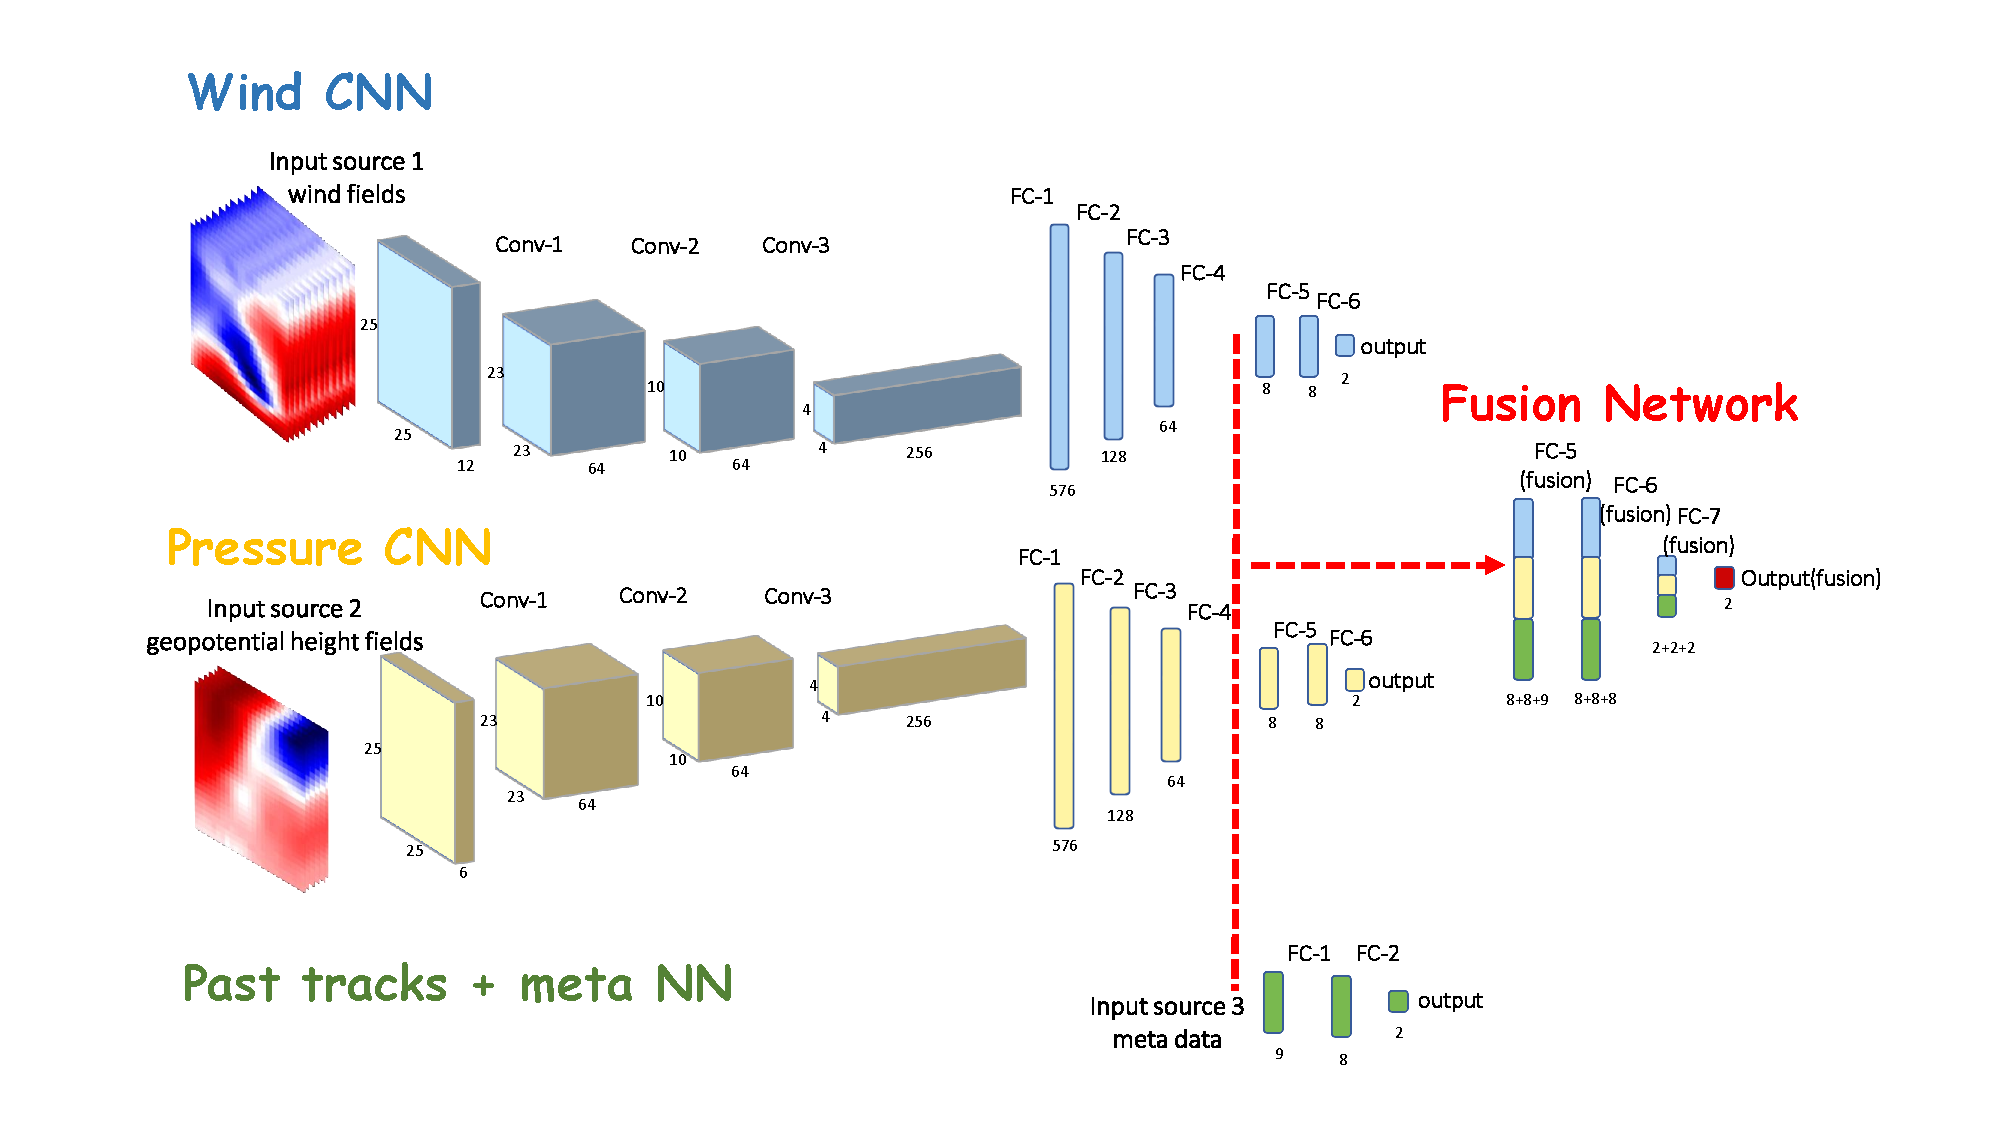
\includegraphics[width=0.8\linewidth]{figs/fusion_network.pdf}
\end{figure}
\end{frame}


\begin{frame}
\frametitle{Train Stream Networks}
\begin{itemize}
	\item  Stage \Rmnum{1}: Train stream networks \\
	\begin{itemize}
		\item Wind CNN
		\begin{itemize}
			\item pretty standard (popular) CNN architecture, like VGG Net \cite{simonyan2014very}
			\item trying from shallow to deep
			\item \textbf{Details:} ReLU, batch norm, adam, batch size=$32$, L2 $coeff.$ = $0.01$, initial learning rate = $0.001$, $He$ initialization \cite{he2015delving}, everything fine tuned... \textbf{No magic!}
		\end{itemize}
	\end{itemize}
\end{itemize}
\begin{figure}
	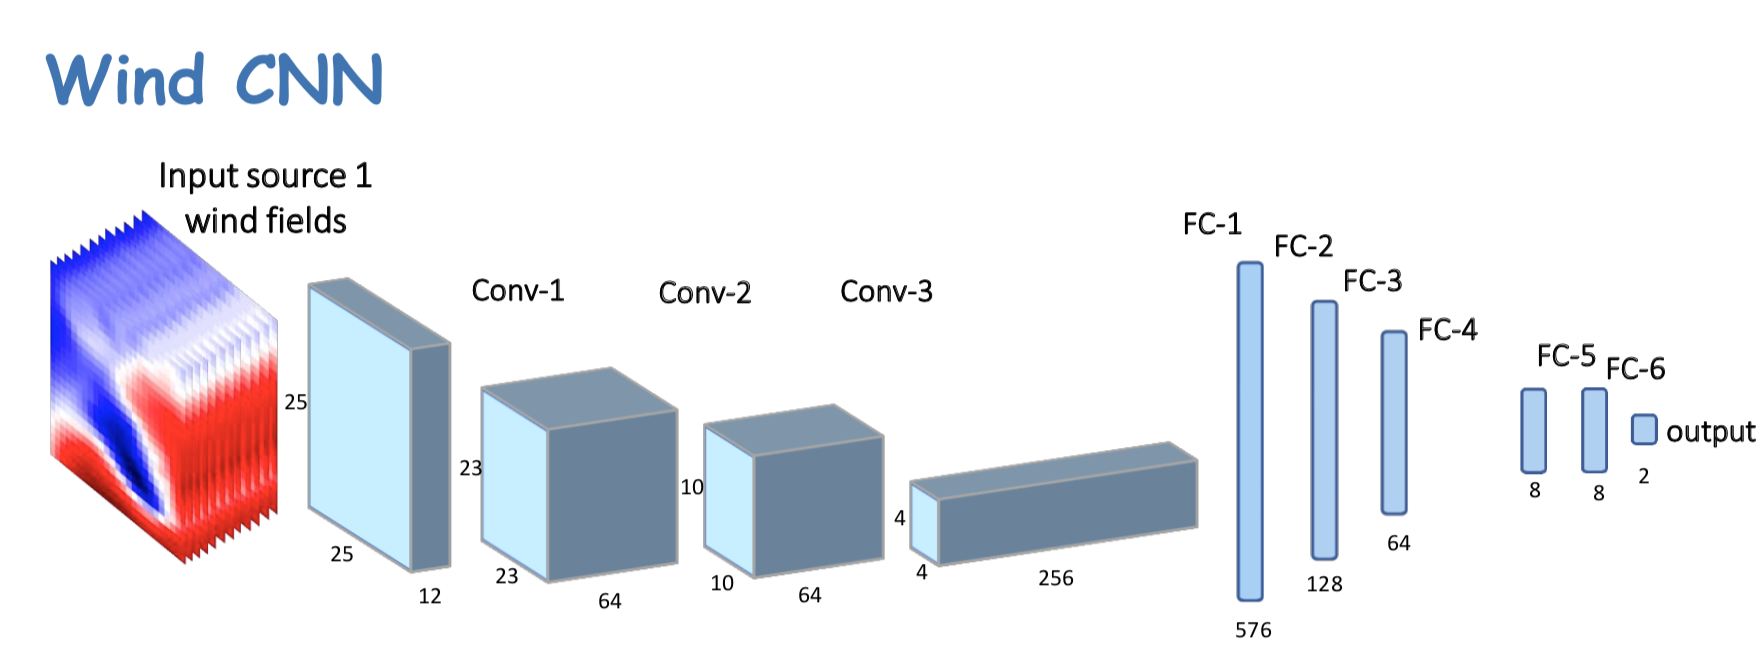
\includegraphics[width=0.8\linewidth]{figs/wind-cnn.png}
\end{figure}
\end{frame}

\begin{frame}
\frametitle{Train Stream Networks}
\begin{itemize}
	\item  Stage \Rmnum{1}: Train stream networks \\
	\begin{itemize}
		\item Pressure CNN
		\begin{itemize}
			\item same principle...
		\end{itemize}
		\item Past tracks + meta NN
			\begin{itemize}
				\item a simple multi-layer perception (MLP)
			\end{itemize}
	\end{itemize}
\end{itemize}
\begin{figure}

	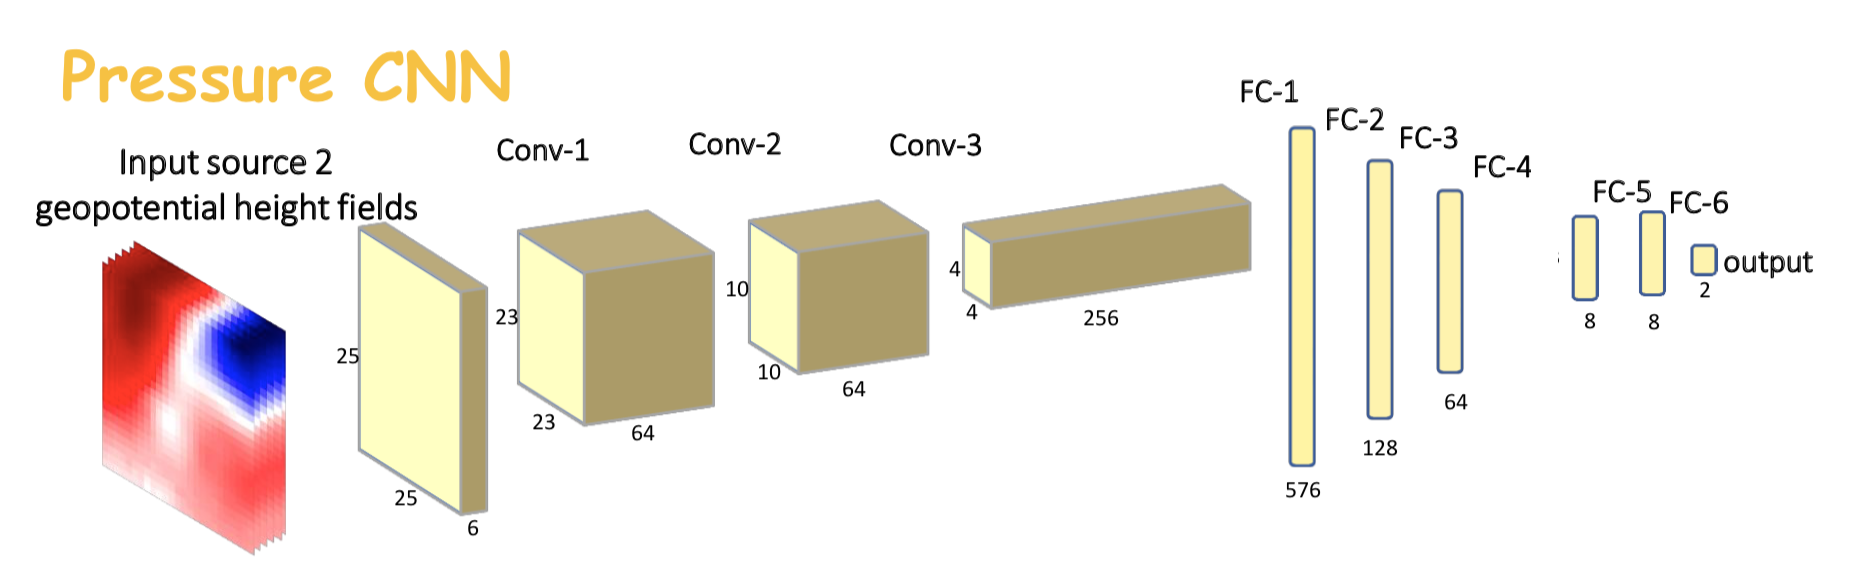
\includegraphics[width=0.65\linewidth]{figs/pressure-cnn.png} \\
	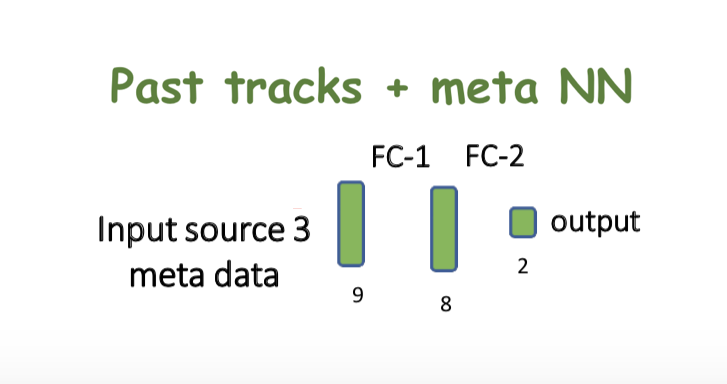
\includegraphics[width=0.32\linewidth]{figs/meta-nn.png}
\end{figure}
\end{frame}



\begin{frame}
\frametitle{Train Fusion Network}
\begin{itemize}
	\item  Stage \Rmnum{2}: Train the fusion network \\
\end{itemize}
\begin{figure}
	
	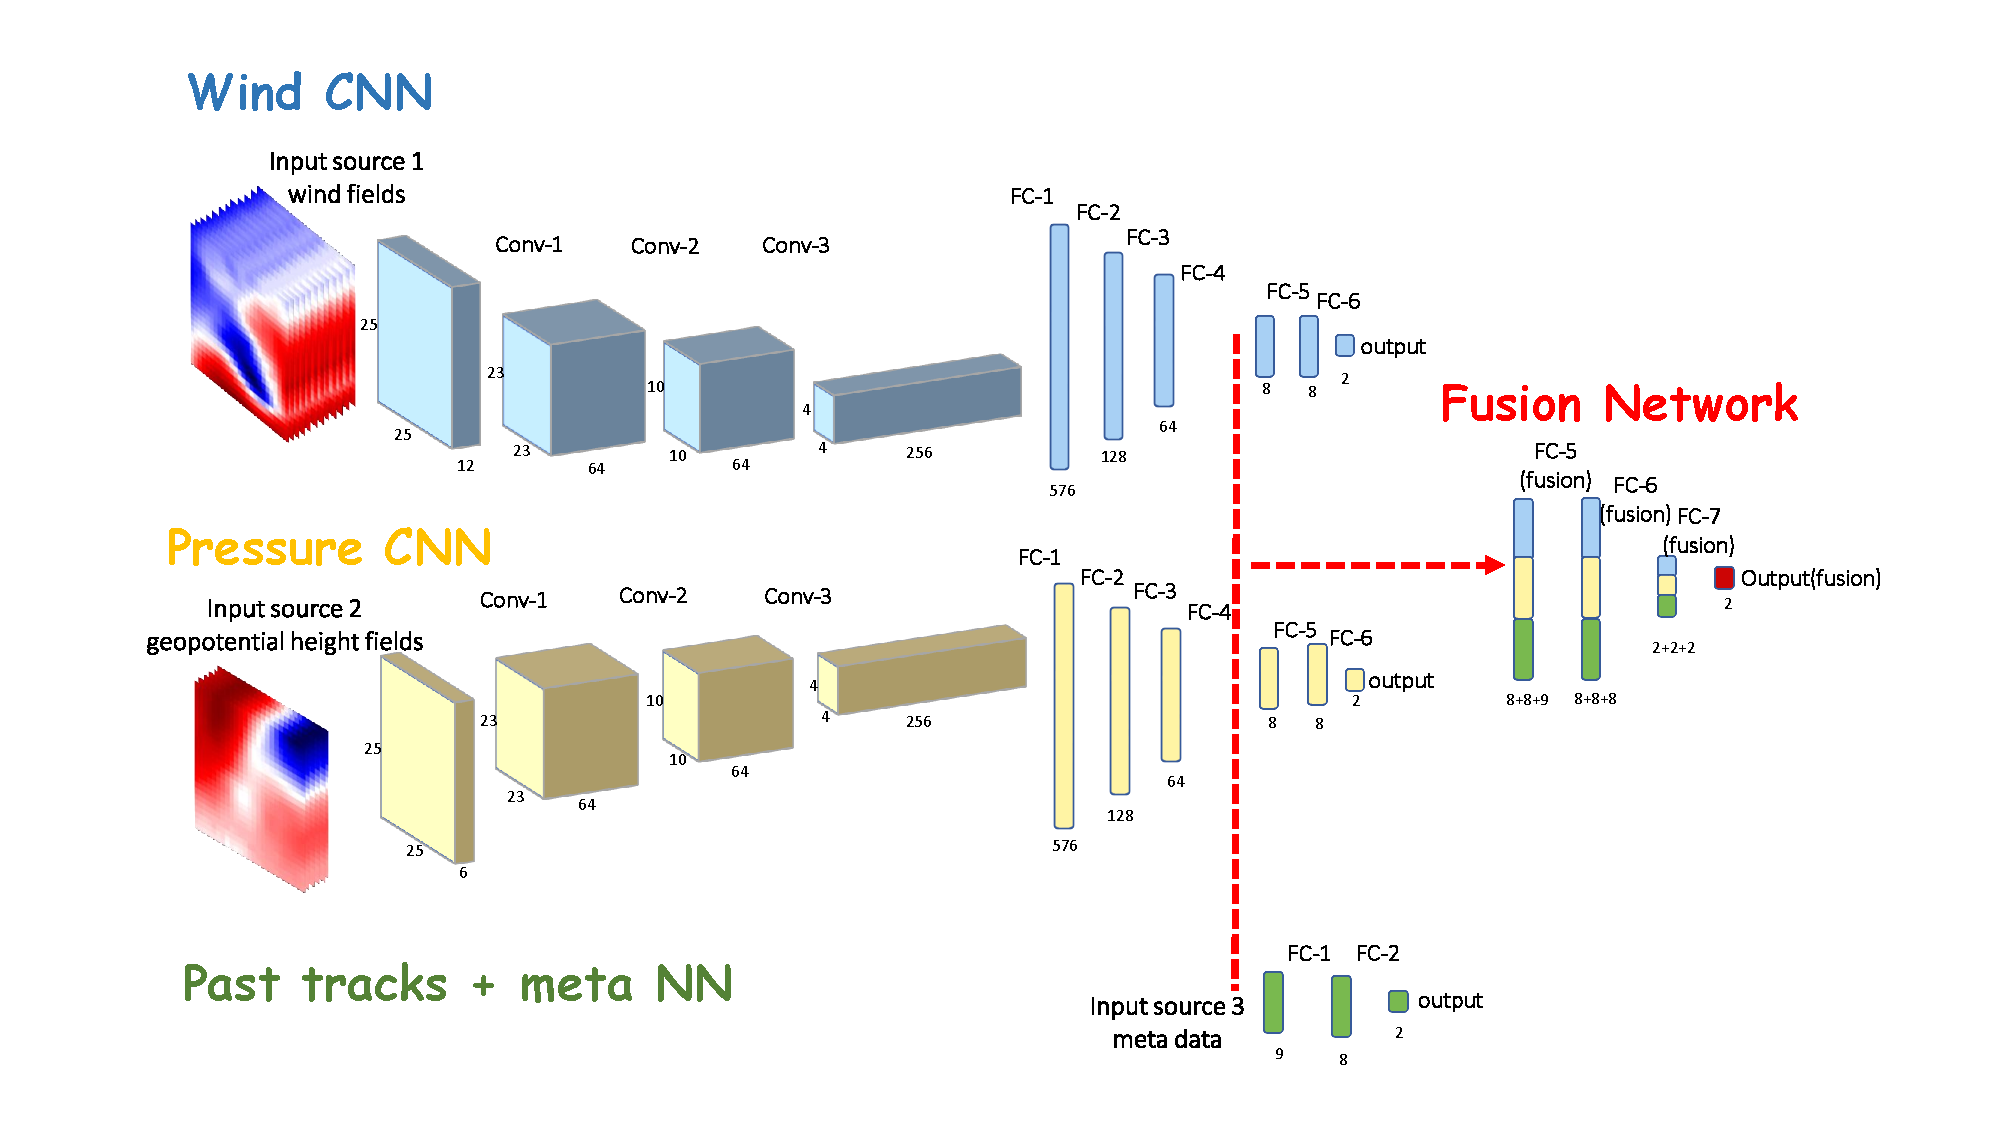
\includegraphics[width=0.8\linewidth]{figs/fusion_network.pdf} \\
	
\end{figure}
\end{frame}

\begin{frame}
\frametitle{Train Fusion Network}
\begin{itemize}
	\item  Stage \Rmnum{2}: Train the fusion network \\
	\begin{itemize}
		\item  zoom in fusion layers
		\begin{figure}
			\flushleft
			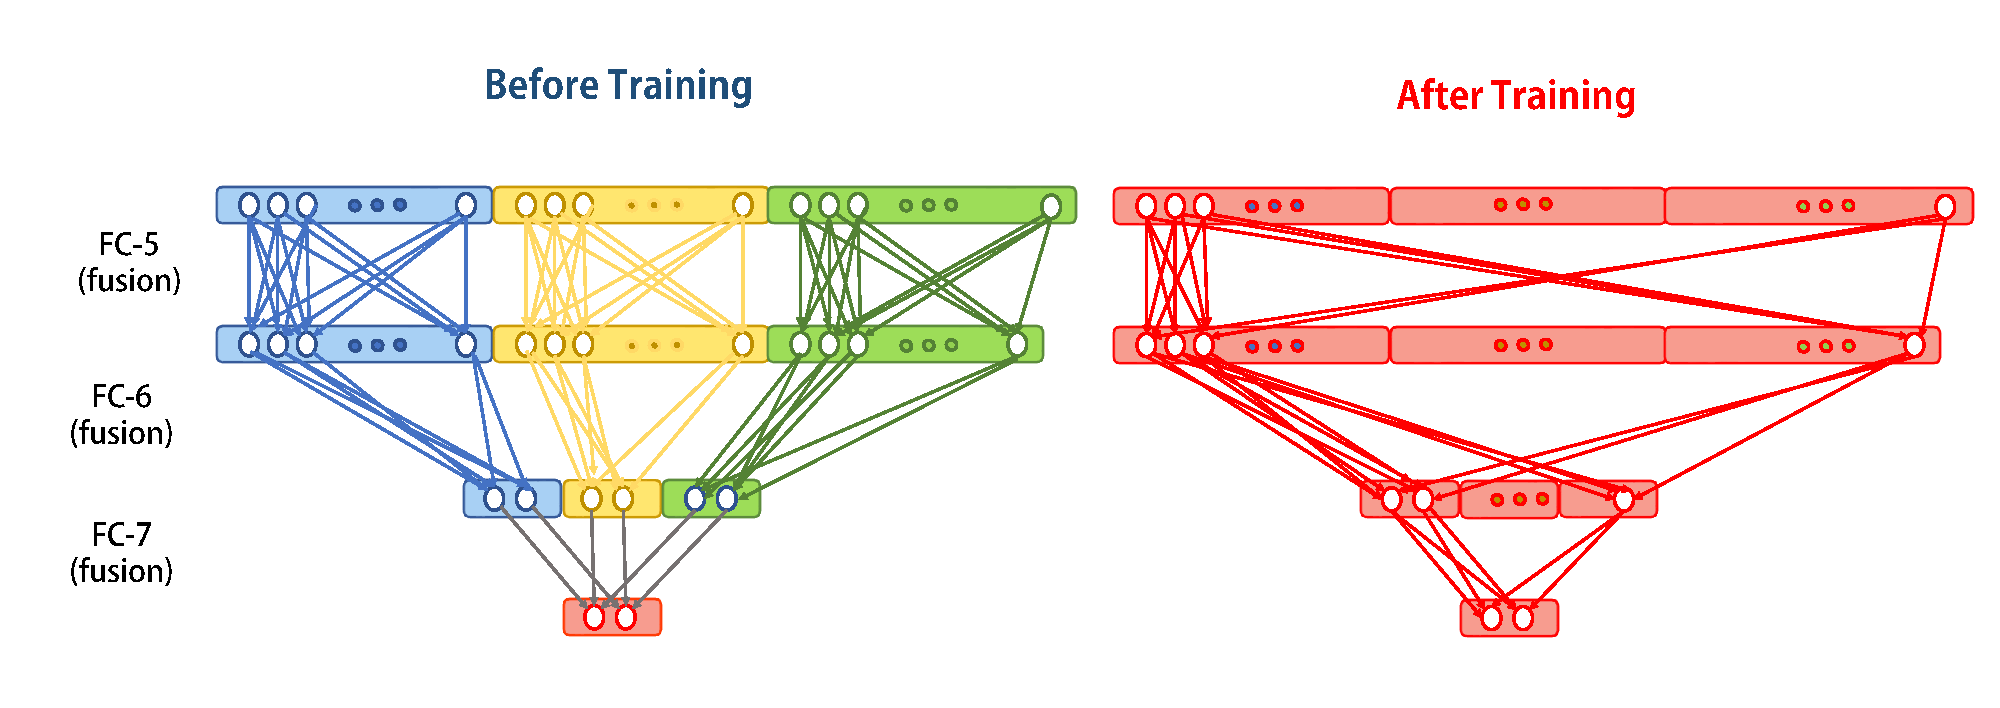
\includegraphics[width=0.65\linewidth]{figs/fusion_details.pdf} \\
		\end{figure}
		\item two-phase optimization:
			\begin{itemize}
				\item first phase: optimize weights only in fusion layers
				\item seconc phase: optimize weights in all layerts
			\end{itemize}
	\end{itemize}
\end{itemize}
\end{frame}

\subsection{Fusion Network Training Framework}
\begin{frame}
\frametitle{Outline} % Table of contents slide, comment this block out to remove it
\tableofcontents[currentsubsection] % Throughout your presentation, if you choose to use \section{} and \subsection{} commands, these will automatically be printed on this slide as an overview of your presentation
\end{frame}
\begin{frame}
\frametitle{Input preprocessing}
\begin{itemize}
	\item  the entire dataset into train (60\%) / validation (20\%) / test (20\%)
	\item separate all the storms into the three bins to avoid data leakage
	\item input data standardized by subtracting mean value then dividing by the standard variation of each layer, computed on the training set, from each feature
\end{itemize}
\end{frame}

\begin{frame}
\frametitle{Training}
Let $D = \{(x_w^1, x_p^1, x_{0d}^1, loc_t^1, loc_{t+\delta t}^1), ..., (x_w^n, x_p^n, x_{0d}^n, loc_t^n, loc_{t+\delta t}^n)\}$ be the labeled data; with $x_w^i$, $x_p^i$, $x_{0d}^i$ denoting wind fields, pressure fields, 0d features respectively and $loc_t^i$, $loc_{t+\delta t}^i$ corresponding to the ground truth location at current time and after $\delta t$ time. $\delta t$ can be 6 hours, 12 hours, 18 hours, 24 hours... depending on the specific forecasting task. 
\end{frame}

\begin{frame}
\frametitle{Training}
	\begin{itemize}
		\item  Stage \Rmnum{1}: Train the stream networks \\ let $F_{wind}$ be the mapping function of Wind CNN, the network parameters are marked as $\theta_w$, $F_{transform}$ is the transformation function from differences in latitude and longitude to distance. The training of Wind CNN is carried out by optimizing on the loss (MSE) between the forecast storm location and the corresponding ground truth location 
		\begin{equation}
		\label{eq}
		L(\theta_w) = \frac{1}{n}\sum_{i=1}^{n} \left \| {F_{transform}((F_{wind}(x_w^i; \theta_w)} + loc^i_{t} ) - loc^i_{t+\delta t} ) \right \| ^2
		\end{equation}
		Where n is the total number of instances. Training the Pressure CNN and Past tracks + meta NN can be performed analogously.
	\end{itemize}
\end{frame}

\begin{frame}
\frametitle{Training}
\begin{itemize}
	\item  two-phase manner
	\begin{itemize}
		\item  Let $F_{f}$ be the function of fusion network, $\theta_{f}$, $\theta_{s}$ be parameters of fusion layers and of stream layers. In the first phase, optimize only the weights in the fusion layers (keeping the weights of the stream layers intact). The first phase's loss function would be:
		
		\begin{equation}
		\label{eq_fusion_1}
		L(\theta_{f}) = \frac{1}{n}\sum_{i=1}^{n} \left \| {F_{transform}((F_{f}(x_w^i, x_p^i, x_{0d}^i; \theta_{f})} + loc^i_{t} ) - loc^i_{t+\delta t} ) \right \| ^2
		\end{equation}
		\item In the second phase, let the weights in the whole network be equally optimized. The second phase's loss function would be:
		\begin{equation}
		\label{eq_fusion_2}
		L(\theta_{f}, \theta_{s}) = \frac{1}{n}\sum_{i=1}^{n} \left \| {F_{transform}((F_{f}(x_w^i, x_p^i, x_{0d}^i; \theta_{f}, \theta_{s})} + loc^i_{t} ) - loc^i_{t+\delta t} ) \right \| ^2
		\end{equation}
		
	\end{itemize}
\end{itemize}
\end{frame}

\section{Experiments}
\begin{frame}
\frametitle{Outline} % Table of contents slide, comment this block out to remove it
\tableofcontents[currentsubsection] % Throughout your presentation, if you choose to use \section{} and \subsection{} commands, these will automatically be printed on this slide as an overview of your presentation
\end{frame}

\subsection{Selecting Network Configurations}
\begin{frame}
\frametitle{Experiments}
\framesubtitle{Selecting Stream Network Configuration}
\begin{itemize}
	\item  Four candidates' network configurations for Wind CNN\\
	\begin{itemize}
		\item followed the same generic design
		\item from shalow to deep
	\end{itemize}
\end{itemize}
\begin{figure}
	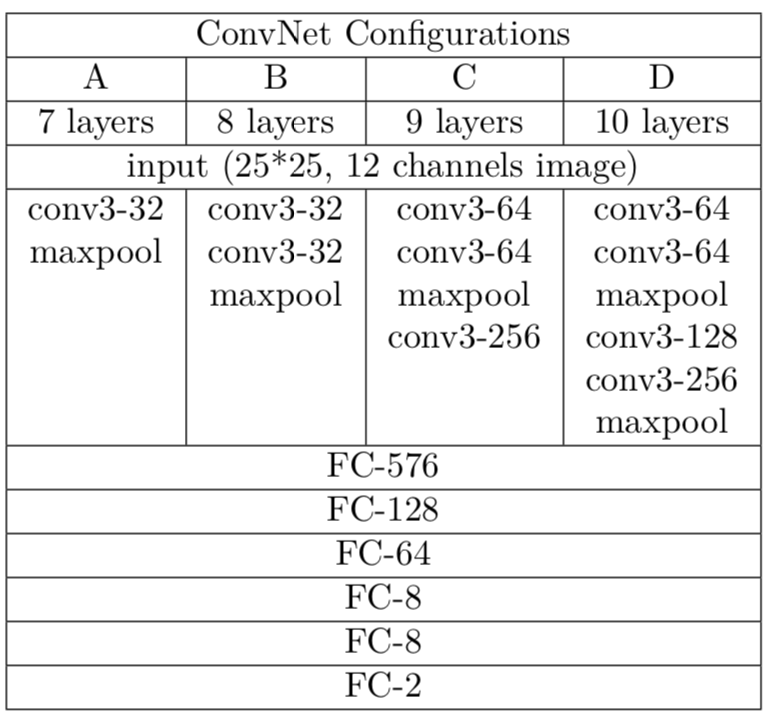
\includegraphics[width=0.4\linewidth, height=0.5\textheight]{figs/candidates.png} \\
\end{figure}
\end{frame}

\begin{frame}
\frametitle{Experiments}
\framesubtitle{Selecting Stream Network Configuration}
\begin{itemize}
	\item  Evaluation results on 24 hours of storm track prediction on the validation set\\

\begin{table}[]
	\centering
	\begin{tabular}{|c|c|c|}
		\hline
		Model& Mean Square Error ($km^2$) & Mean Absolute Error($km$) \\ \hline
		A & 31430.08 & 145.43  \\ \hline
		B & 31761.95 & 146.62  \\ \hline
		C & 31552.91 & 145.5997 \\ \hline
		D & 31772.62 & 146.73 \\ \hline
	\end{tabular}
\end{table}
	\item Adding more temporal parts (storm fields data at the same location at more consecutive time steps to input data)
	\begin{itemize}
		\item  No noticeable improvement\\
	\end{itemize}
\end{itemize}
\end{frame}


\begin{frame}
\frametitle{Experiments}
\framesubtitle{Selecting Fusion Network Configuration}
Two senarios:
\begin{itemize}
	\item  how many layers should be fused?
	\item  Does fusing three streams outperforms fusing two streams or using single stream?
\end{itemize}
\end{frame}

\begin{frame}
\frametitle{Experiments}
\framesubtitle{Selecting Fusion Network Configuration}
\begin{itemize}
	\item  how many layers should be fused?
	\begin{itemize}
		\item Comparison of fusion networks that fuse different number of layers on 24 hours storm track prediction on validation set.
		
	\end{itemize}
	\begin{figure}
		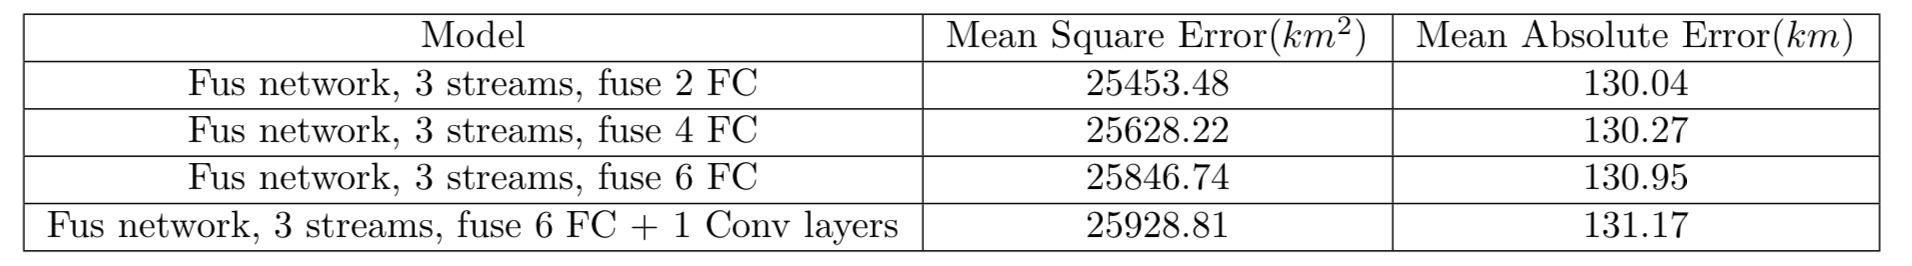
\includegraphics[width=0.95\linewidth]{figs/fusion_1.png} \\
	\end{figure}
	\item  Does fusing three streams outperforms fusing two streams or using single stream?
	\begin{itemize}
		\item Comparison between the fusion network fusing all three streams with networks fusing two streams and single stream networks.
		
	\end{itemize}
	\begin{figure}
		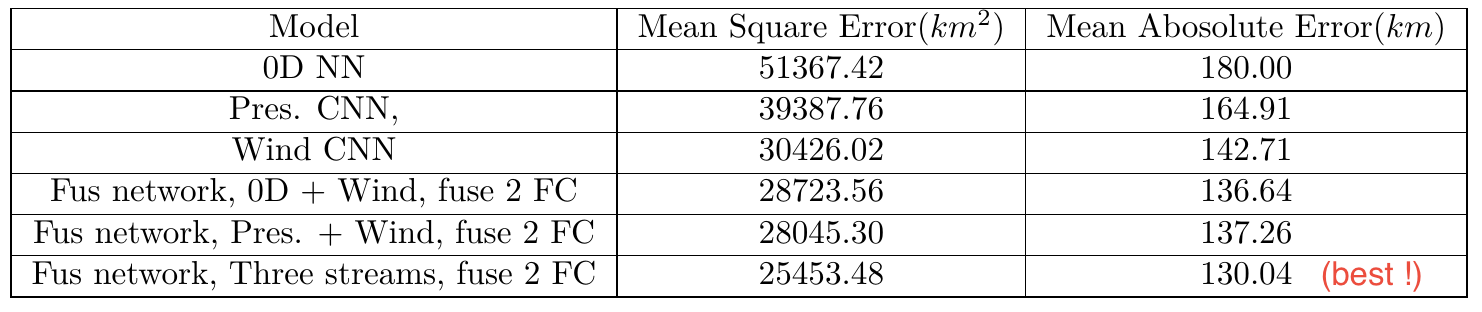
\includegraphics[width=0.8\linewidth]{figs/fusion_2.png} \\
	\end{figure}
\end{itemize}
\end{frame}

\begin{frame}
\frametitle{Experiments}
\framesubtitle{Selecting Fusion Network Configuration}
\begin{figure}
	\caption{24h-forecast results on the test set (storms coming from all oceanic basins), in distance between predicted and real location.}
	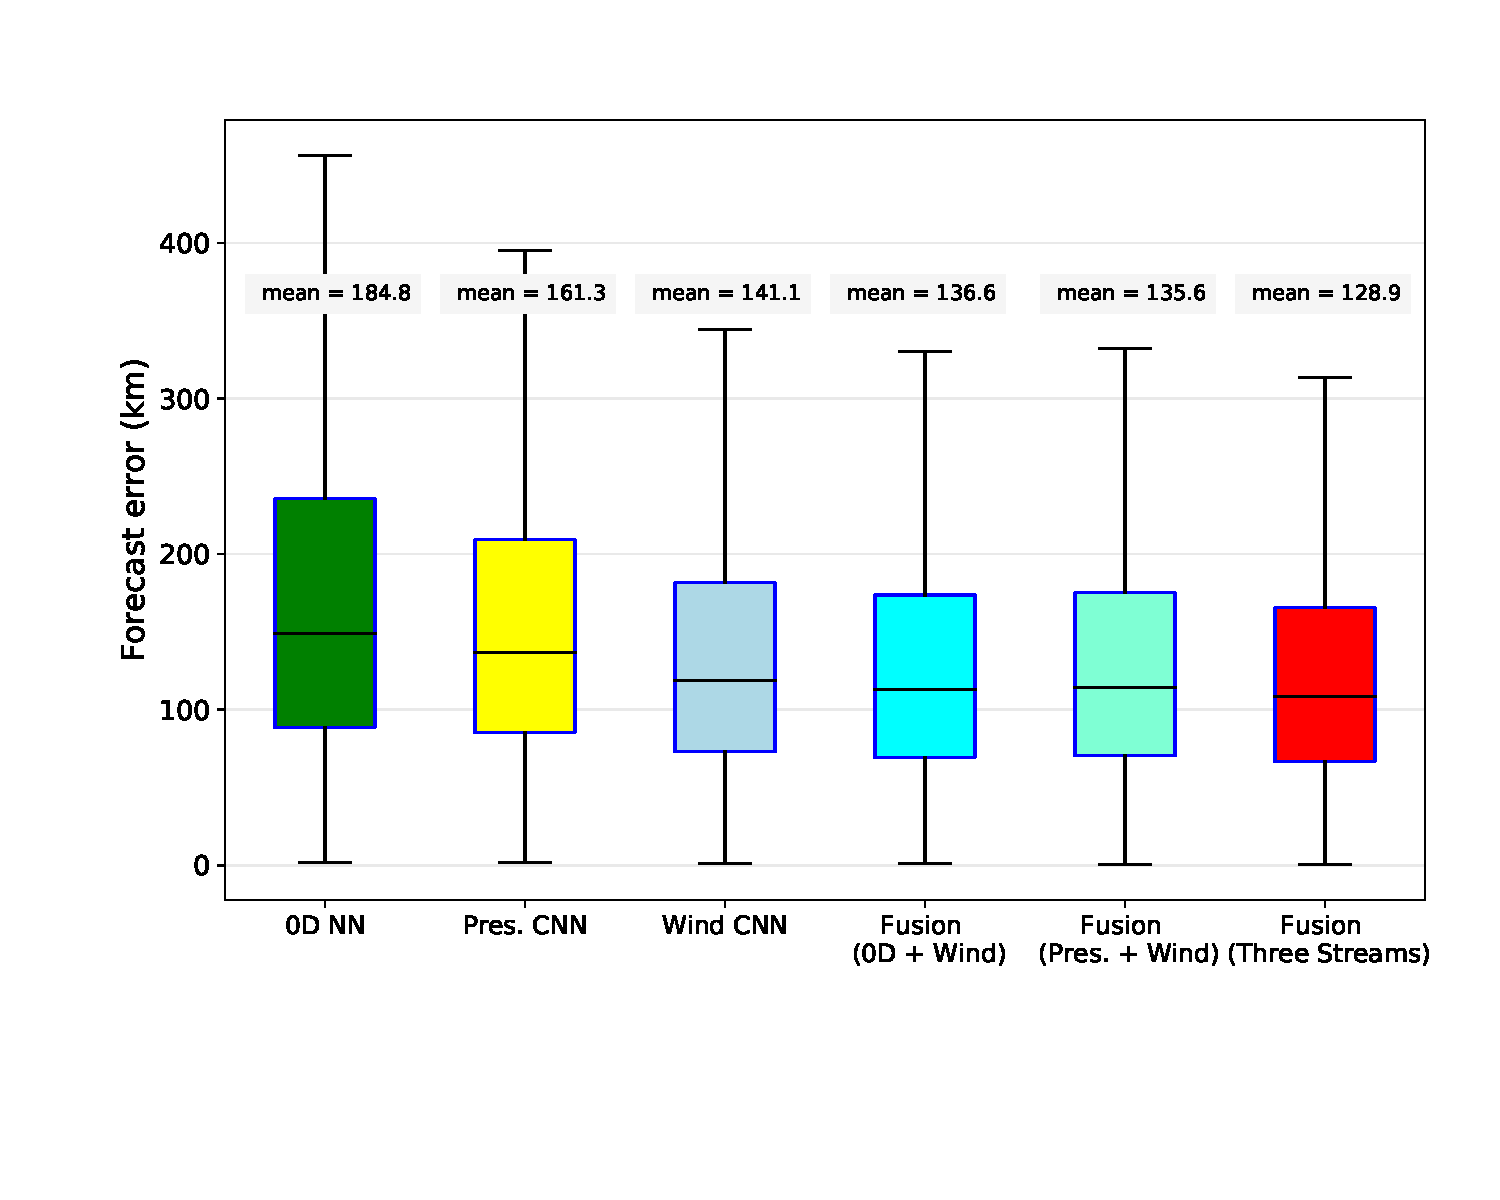
\includegraphics[width=0.75\linewidth]{figs/MAE.pdf} \\
\end{figure}

\end{frame}


\subsection{Comparison with the Existing Forecasting Models}
\begin{frame}
\frametitle{Outline} % Table of contents slide, comment this block out to remove it
\tableofcontents[currentsubsection] % Throughout your presentation, if you choose to use \section{} and \subsection{} commands, these will automatically be printed on this slide as an overview of your presentation
\end{frame}

\begin{frame}
\frametitle{Experiment} 
\framesubtitle{Comparison with the Existing Forecasting Models}
\begin{itemize}
	\item \textbf{Baselines:} A commenly used statisticall model for benchmarking:  Best Track Decay (BCD5)
	\item Also compare with: Official NHC forecast (OCFL). With increased computational power, the performance of OFCL is constantly improving
	
\end{itemize}
\end{frame}


\begin{frame}
\frametitle{Experiments}
\framesubtitle{Comparison with the Existing Forecasting Models}
Quantitative: 
\begin{figure}
	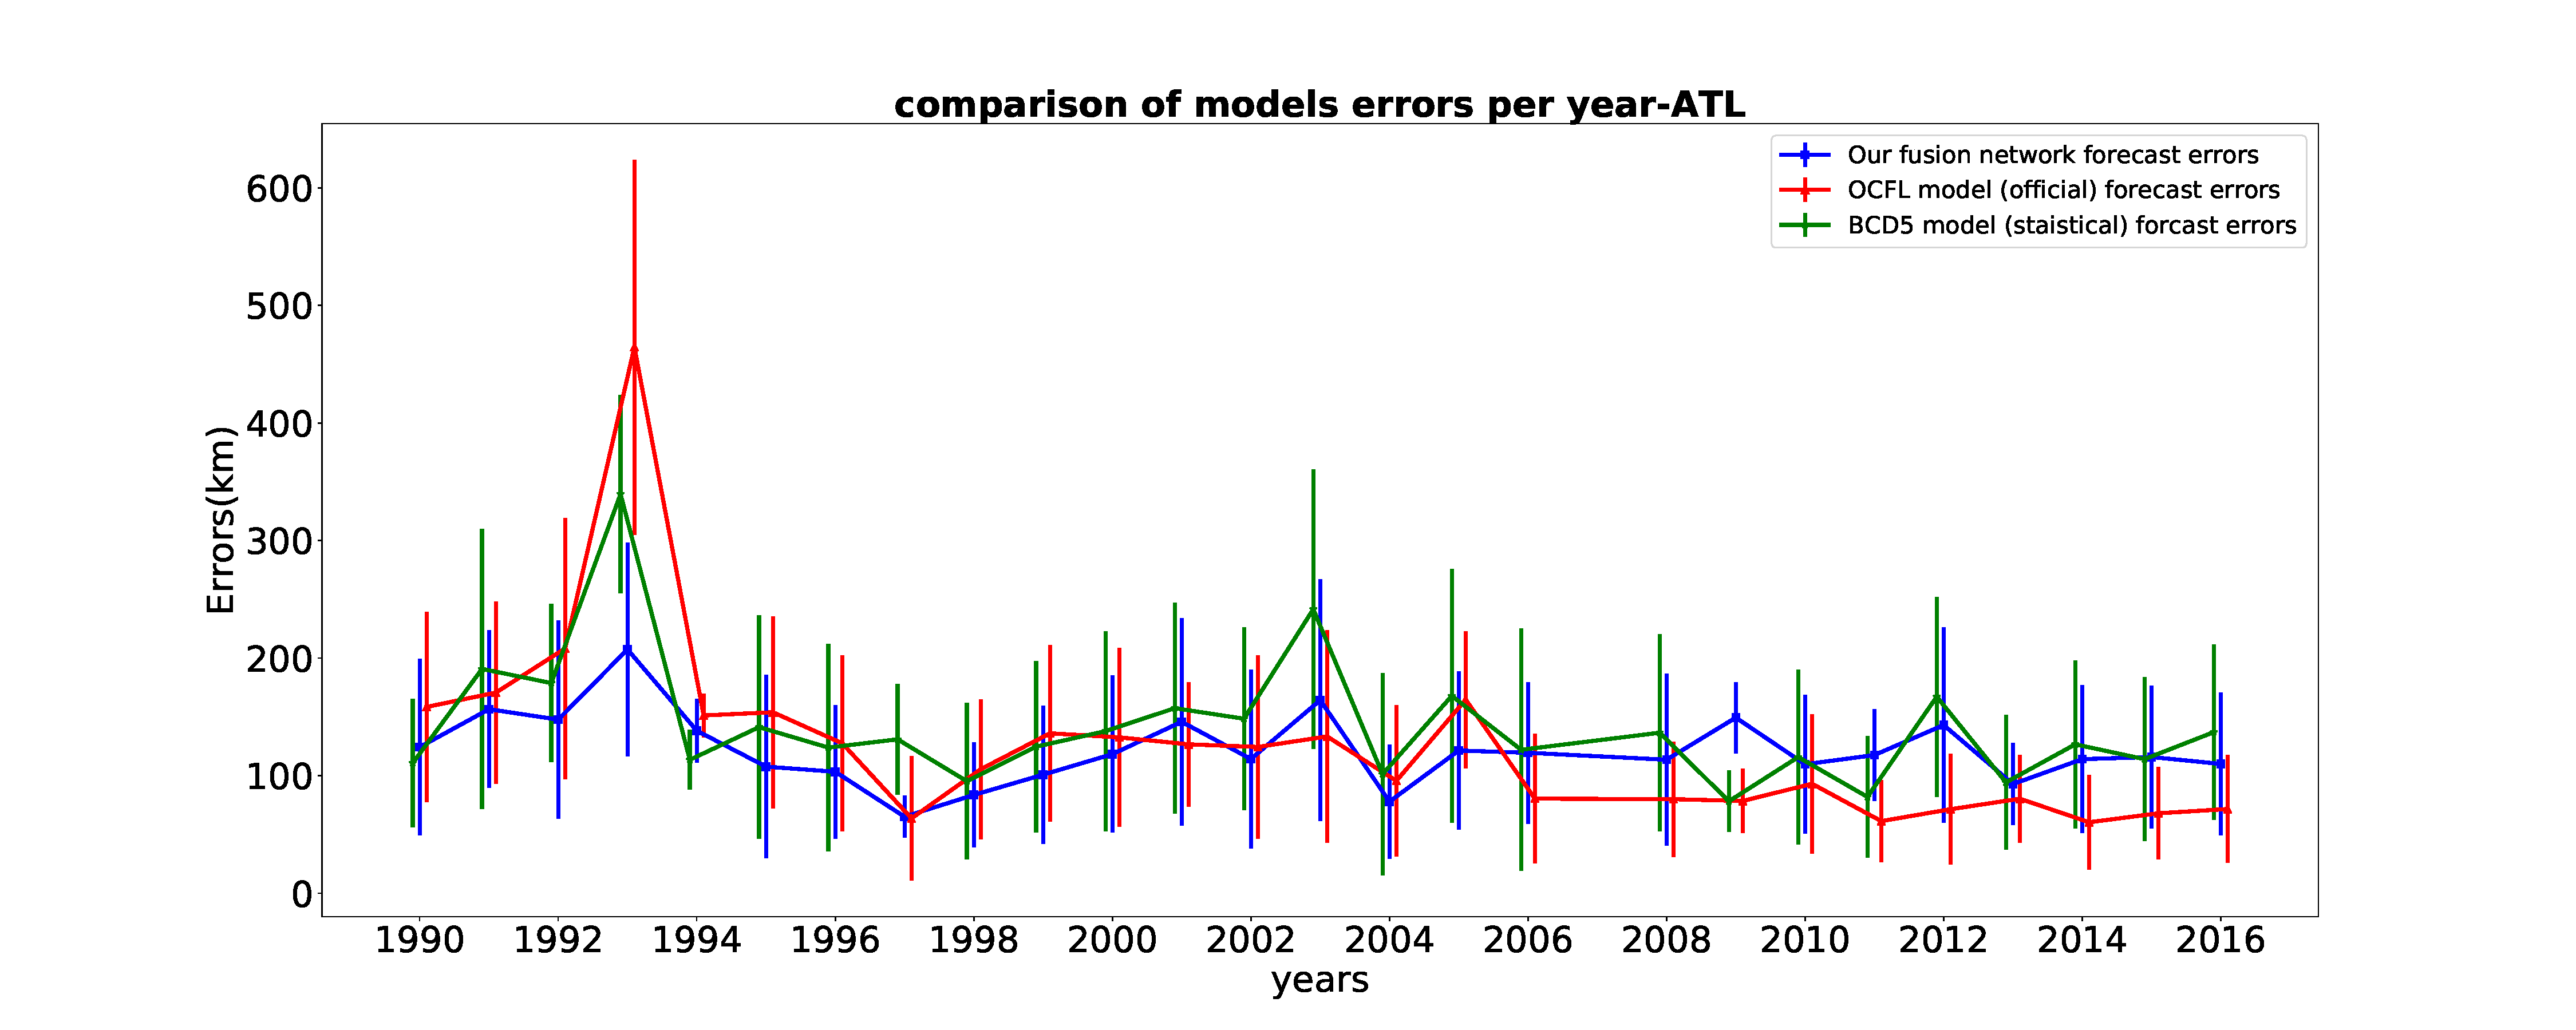
\includegraphics[width=1.0\linewidth]{figs/ATL_comparison_of_models_errors_per_year.pdf}\\
	\caption{The yearly average 24-hours storm track forecasting errors (km) and standard deviation on the test set in Atlantic for our fusion network forecasts(blue), the BCD5 (green) and the OFCL (red), 1989-2016.}
\end{figure}
\end{frame}

\begin{frame}
\frametitle{Experiments}
\framesubtitle{Comparison with the Existing Forecasting Models}
Quantitative: 
\begin{figure}
	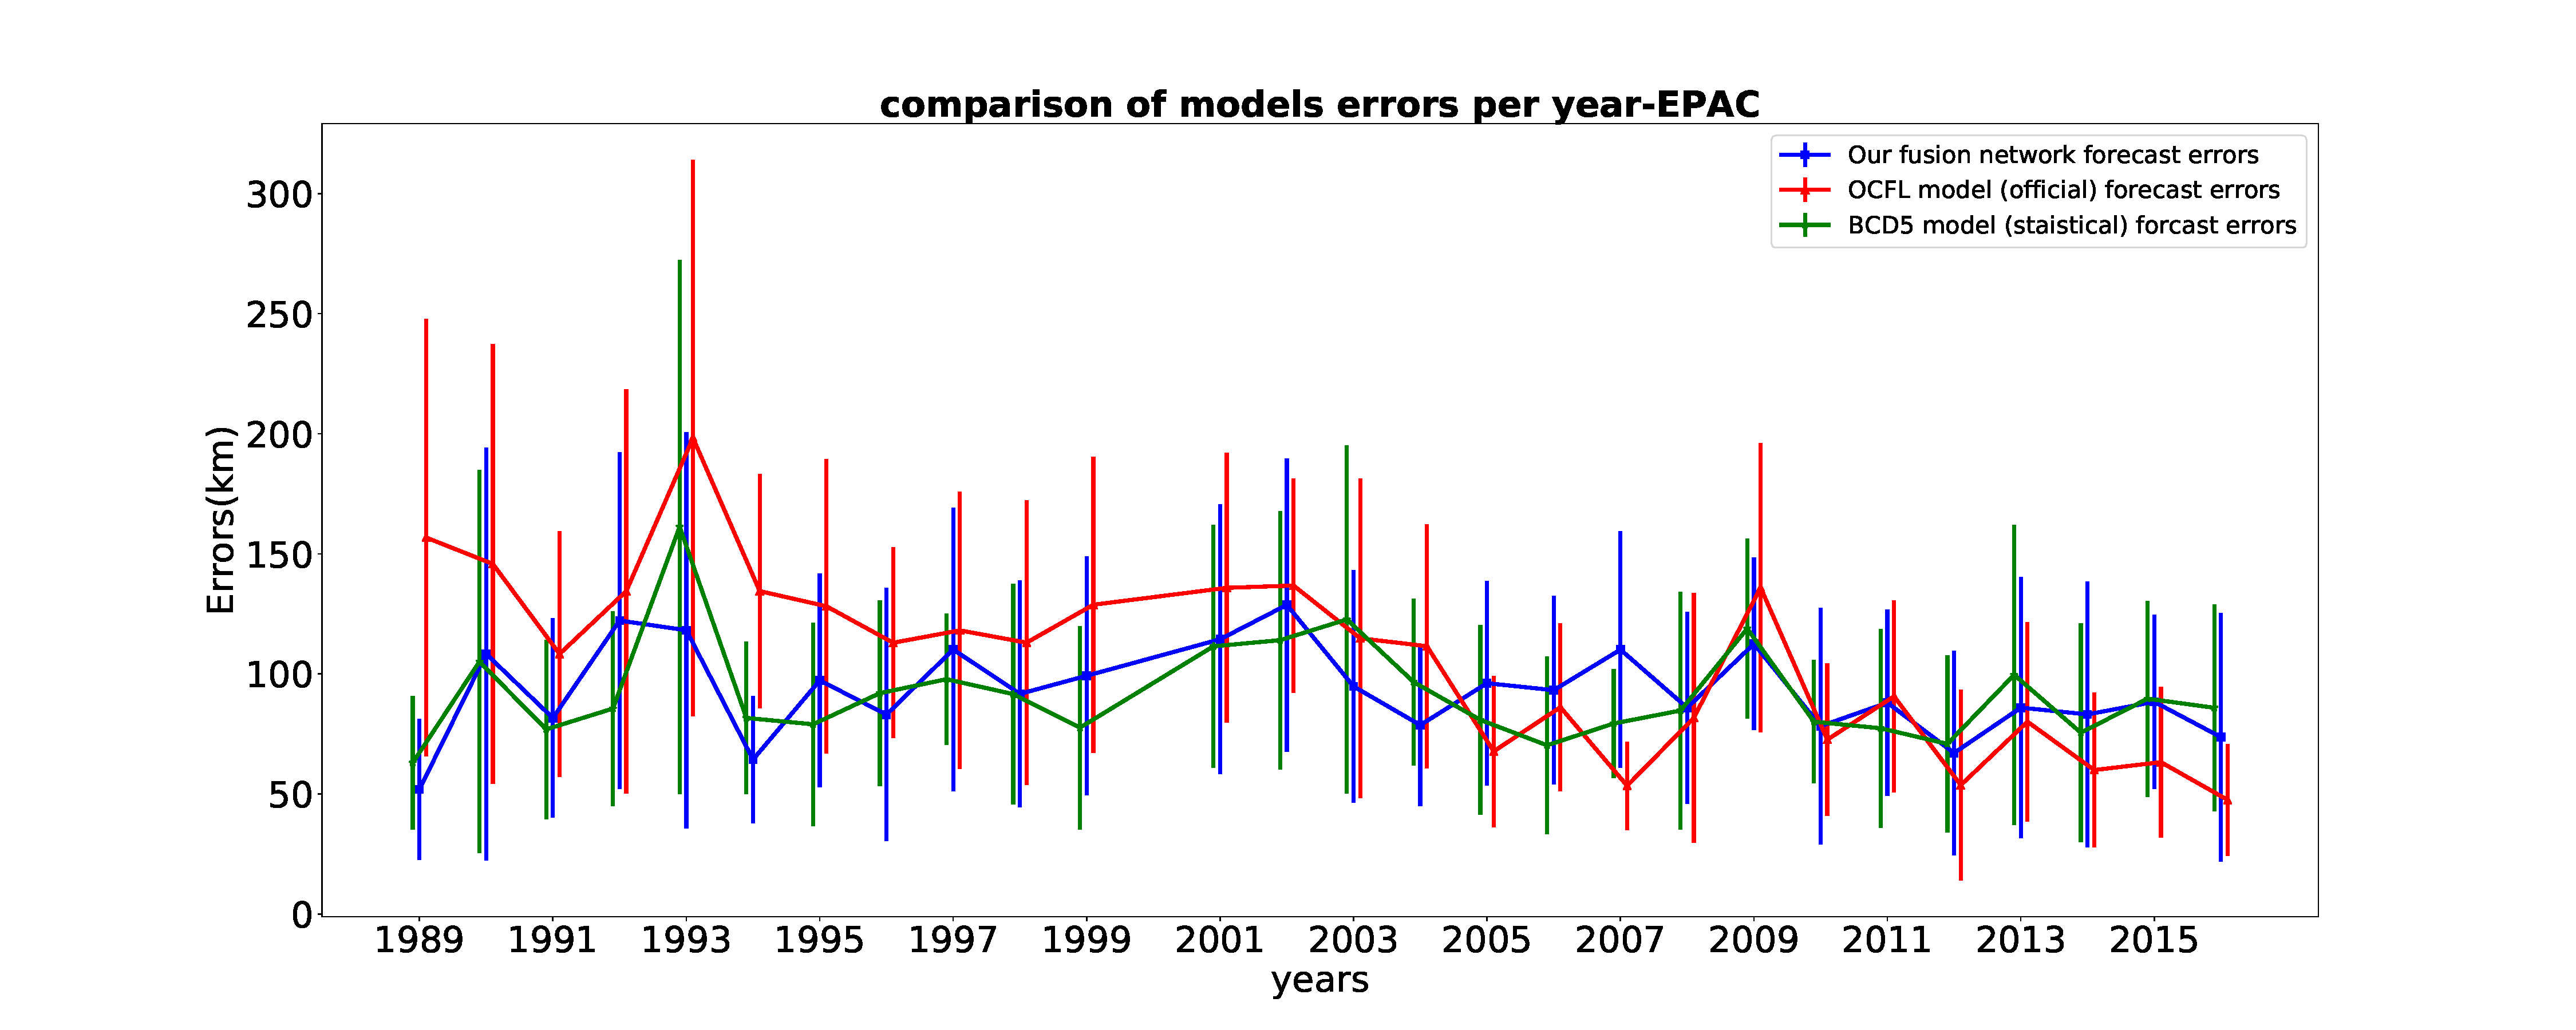
\includegraphics[width=1.0\linewidth]{figs/EPAC_comparison_of_models_errors_per_year.pdf}\\
	\caption{The yearly average 24-hours storm track forecasting errors (km) and standard deviation on the test set in East Pacific for our fusion network forecasts (blue), the BCD5 (green) and the OFCL (red), 1989-2016.}
\end{figure}
\end{frame}

\begin{frame}
\frametitle{Experiments}
\framesubtitle{Comparison with the Existing Forecasting Models}
Quantitative: \\
\begin{itemize}
	\item Mean storm track forecast errors of all years in the two basins (Atlantic and Pacific) on the test set for our fusion network and BCD5 model: 
\end{itemize}

\begin{figure}
	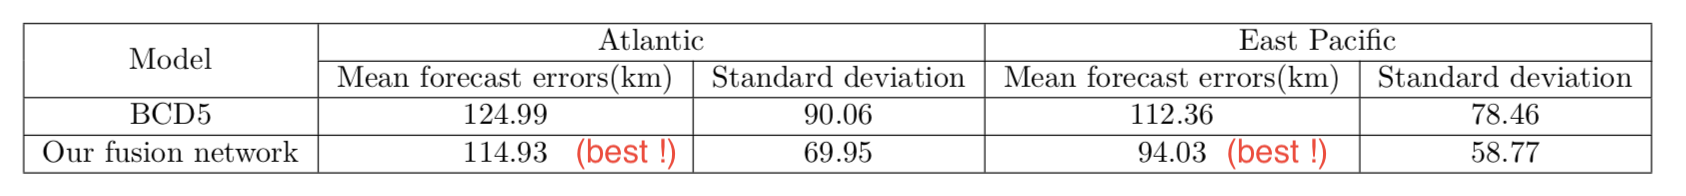
\includegraphics[width=1.0\linewidth]{figs/compare_with_baseline}\\
\end{figure}
\end{frame}

\begin{frame}
\frametitle{Experiments}
\framesubtitle{Comparison with the Existing Forecasting Models}
Qualitative: 

\begin{figure}
	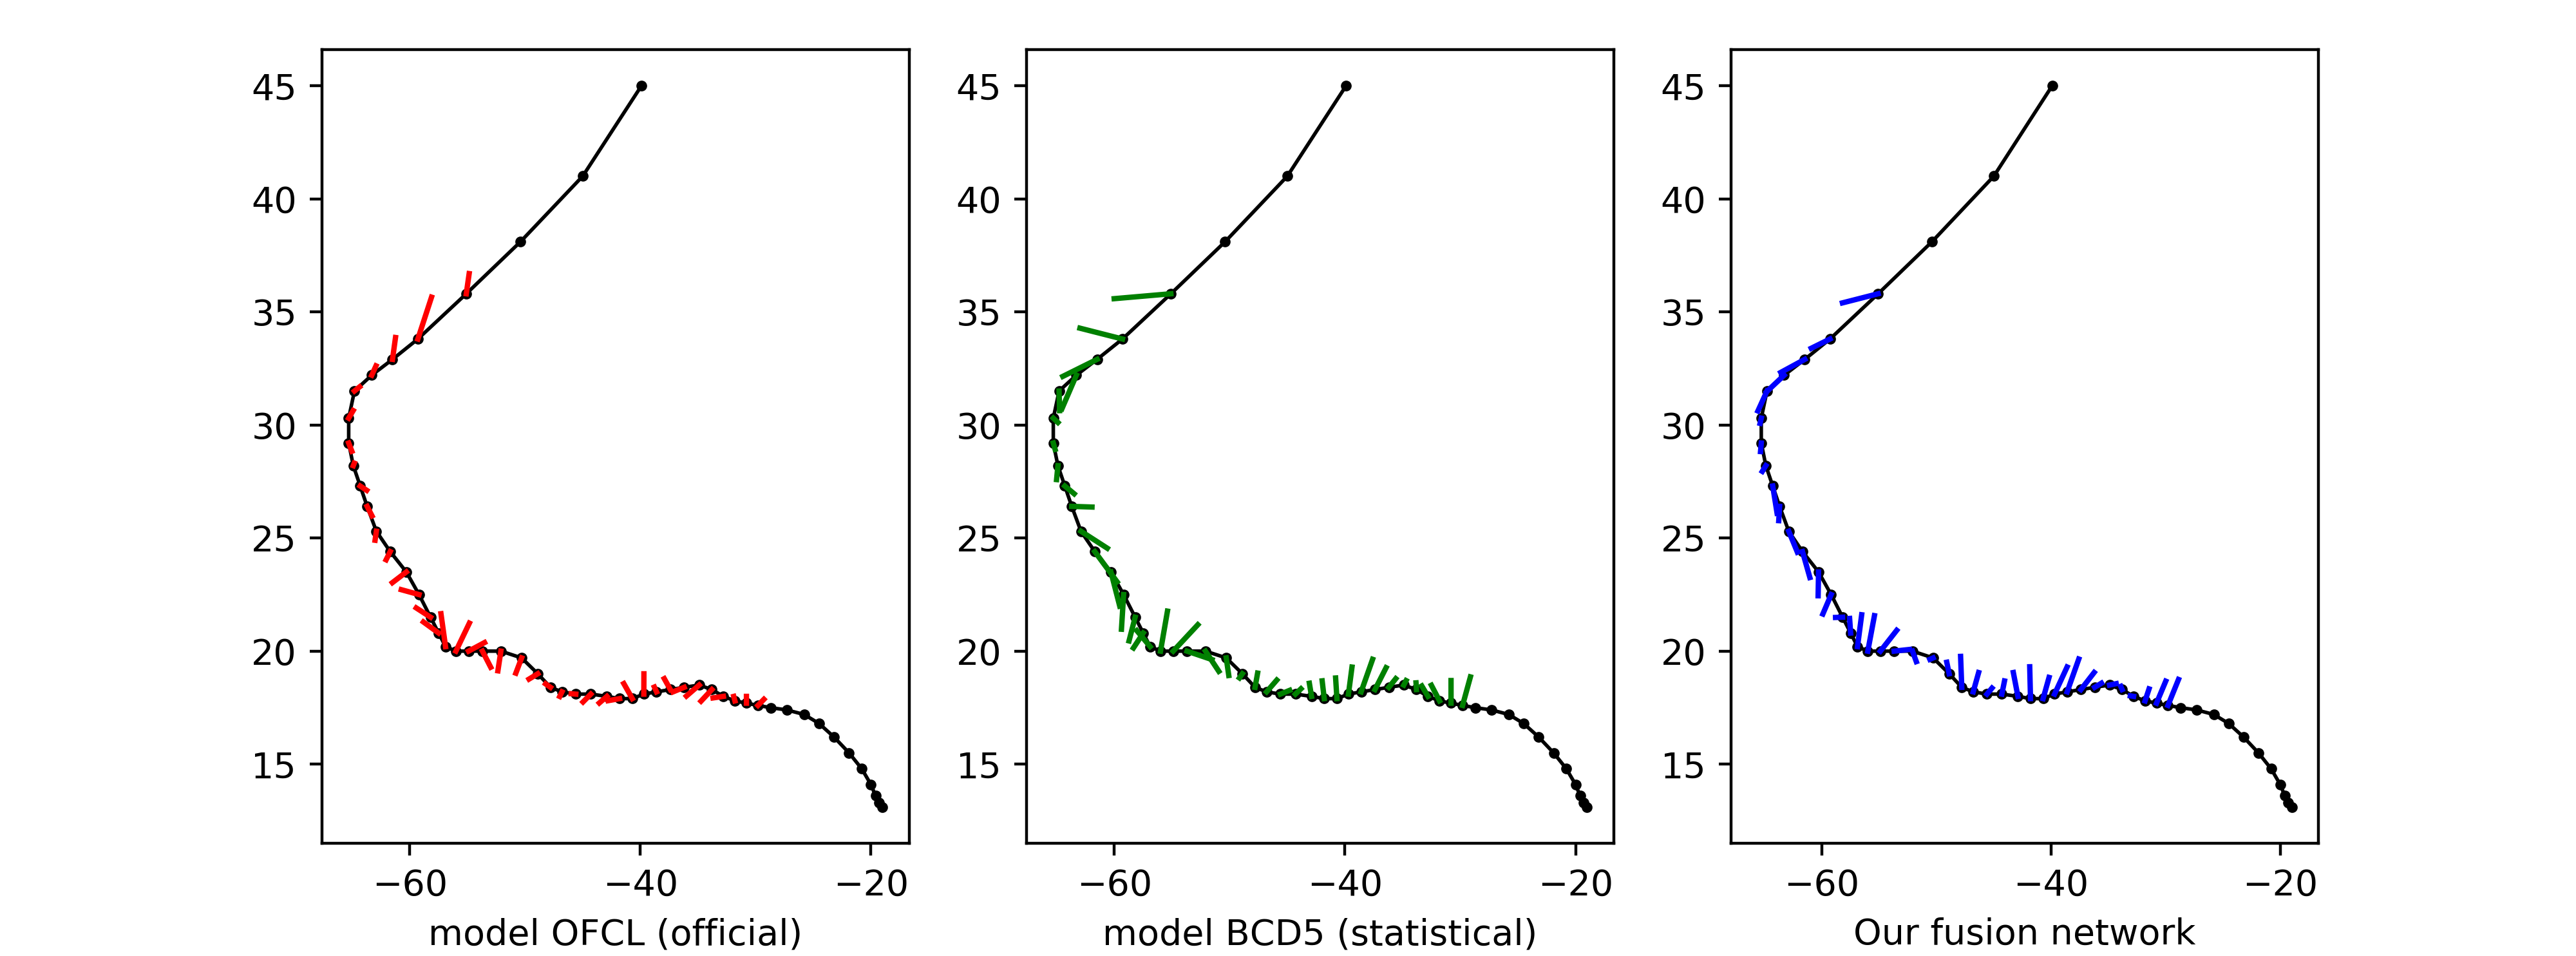
\includegraphics[width=1.0\linewidth]{figs/one_stom_result.png}\\
	\caption{The forecast errors of the three models (left: the OCFL, middle: the BCD5, right: our fusion network) on the Hurricane Ian in 2016}
\end{figure}
\end{frame}




\section{Discussion}
\begin{frame}
\frametitle{Discussion}
\large{Conclusion:}

\begin{itemize}
	\item  Proposed a promising deep learning framework for storm track forecasting
	\item  Coupled different types of data (wind fields, pressure fields, past tracks and other handcrafted data) into our fusion model
	\item  our model outperforms the BCD5 model
	\item  our model can help to enhance the official forecast, even its forecast errors are larger than the OFCL model.
\end{itemize} 
\end{frame}

\section{Discussion}
\begin{frame}
\frametitle{Discussion}
\large{What's next?}

\begin{itemize}
	\item  Design an algorithm that could effectively learn information from high-dimensional tensor data.
	\item  Try unsupervised learning algorithms (e.g. clustering)
	\item  Apply multi-target learning
\end{itemize} 
\end{frame}

\begin{frame}
\Huge{\centerline{THANK YOU}}
\end{frame}


\bibliographystyle{apalike}   
\bibliography{presentation.bib}
\end{document}